\chapter{Alphabet 1}\label{alphabet-1}

\emph{We'll start with some simple sentences right away. Russian does
not have articles, nor does it normally use the verb ``to be'' in the
Present tense.}

An em-dash is used instead of ``the verb ``to be'' between the two
nouns: «Мокка --- кофе» (``A mocha is coffee'').

Russian uses a version of the Cyrillic Alphabet. Many letters look
similar to their Latin counterparts. As Cyrillic typography was
remodeled around 300 years ago, both alphabets have a similar style.

For information on how to install a Russian keyboard layout, please
click \href{https://www.duolingo.com/comment/11449014}{here}.

To switch Duolingo from Latin transliterations to Cyrillic, click the
little \textbf{Aa-Яя} switch near the top of the screen during a lesson.

\section{Letters and Sounds}\label{letters-and-sounds}

\textbf{К}, \textbf{О}, \textbf{М}, \textbf{Т}, \textbf{А} sound similar
to their Latin counterparts (to be more precise, ``о'' is the sound in
``more''). However, in handwriting and typed italics, the letter
\textbf{Т} can look rather like a lower case `m' in the Latin alphabet.
E.g. in the verb \emph{просить} (to ask for, to request), \emph{т} = t.

\textbf{Е} actually sounds more like ``ye'', as in ``yell'', not as in
``Hear ye, hear ye!'' (this will work for now; it's more complicated
after a consonant).

\textbf{В} sounds like `v', \textbf{Б} sounds like `b'. \textbf{Н} is
``n'' and \textbf{И} is ``i'' ('eeh'). The remaining letters are
included in the table below:

\begin{longtable}[]{@{}lll@{}}
\toprule
Ёё$^0$ (\textbf{you}r) & Вв (\textbf{v}ase) & Бб
(\textbf{b}ed)\tabularnewline
Ээ (r\textbf{e}d) & Нн$^1$ (\textbf{n}ap) & Дд$^1$
(\textbf{d}ab)\tabularnewline
Уу (s\textbf{oo}n) & Хх$^2$ (Ba\textbf{ch}) & Гг
(\textbf{g}ap)\tabularnewline
Ии (m\textbf{ee}t) & Йй (\textbf{y}es) & Лл$^1$
(ni\textbf{l})\tabularnewline
Юю (\textbf{you}) & Рр (trilled R) & Пп (\textbf{p}oor)\tabularnewline
Ыы$^3$ (h\textbf{i}t) & Сс (\textbf{S}am) & Зз
(\textbf{z}ebra)\tabularnewline
Яя (\textbf{ya}rd) & Фф (\textbf{ph}oton) & Цц
(ca\textbf{ts})\tabularnewline
Жж$^4$ (sei\textbf{z}ure) & Шш$^4$ (\textbf{sh}un) & Щщ$^4$\tabularnewline
\begin{minipage}[t]{0.32\columnwidth}\raggedright\strut
Чч (\textbf{ch}eer)\strut
\end{minipage} & \begin{minipage}[t]{0.32\columnwidth}\raggedright\strut
\strut
\end{minipage} & \begin{minipage}[t]{0.32\columnwidth}\raggedright\strut
Ъ and Ь$^5$\strut
\end{minipage}\tabularnewline
\bottomrule
\end{longtable}

\begin{itemize}
\tightlist
\item
  $^0$ \textbf{Ёё} The umlaut-like double dots are optional in writing.
  Syllables containing this letter are always stressed.
\item
  $^1$ \textbf{т, д, н, л} are pronounced near your teeth
\item
  $^2$ \textbf{х}('kh') is somewhat similar to the H in ``hue''. It is like
  making the ``sh'' sound, only it is pronounced where you make the
  ``K'' sound.
\item
  $^3$ \textbf{ы} has no equivalent in English. It is an ``eeh''-like
  sound, but less distinct, sounds closer to ``e'' in ``lover'', and has
  your tongue deeper that in ``heat'' or ``hit''.
\item
  $^4$ for \textbf{ш} and \textbf{ж} your tongue is lower than in English
  and slightly bent back. \textbf{Щ} has all your tongue raised---it is
  a longer and more hissy sound. \textbf{Ч} corresponds to \textbf{щ}
  (i.e. a bit different than ``ch'')
\item
  $^5$ \textbf{ъ} and \textbf{ь} are separators and have no sound.
\end{itemize}

\textbf{Л} can have a flat top, like \textbf{П}, or a pointy top like
\textbf{А} (it comes from the Greek $ \Lambda$). Д and Л have a similar top in
many fonts, though it's up to the designer. Handwritten \textbf{Д} looks
like \emph{D}, and \textbf{д} like a \emph{g} or a \emph{д} (the last
two affect the italic shapes).

An Italic \textbf{Г} in lower case usually looks this: \emph{г}.

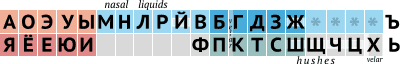
\includegraphics{img/9BB1fM4.png}

That's it with the introduction! We will discuss reading words in more
detail in later skills.

P.S. In our notes, we use an accute accent to show you the stress (e.g.,
р\'{а}дио). It is a standard practice in Russian textbooks for little
children or foreign learners---and, generally, the most common way of
marking the position of the stress.
